\documentclass[landscape,a1paper,fontscale=0.292]{baposter}

\usepackage{times}
\usepackage{calc}
\usepackage{url}
\usepackage{graphicx}
\usepackage{amsmath}
\usepackage{amssymb}
\usepackage{relsize}
\usepackage{multirow}
\usepackage{booktabs}

\usepackage{graphicx}
\usepackage{multicol}
\usepackage[T1]{fontenc}
\usepackage{ae}

\usepackage{wrapfig}

\graphicspath{{images/}}


 %%%%%%%%%%%%%%%%%%%%%%%%%%%%%%%%%%%%%%%%%%%%%%%%%%%%%%%%%%%%%%%%%%%%%%%%%%%%%%%%
 % Multicol Settings
 %%%%%%%%%%%%%%%%%%%%%%%%%%%%%%%%%%%%%%%%%%%%%%%%%%%%%%%%%%%%%%%%%%%%%%%%%%%%%%%%
 \setlength{\columnsep}{0.7em}
 \setlength{\columnseprule}{0mm}


 %%%%%%%%%%%%%%%%%%%%%%%%%%%%%%%%%%%%%%%%%%%%%%%%%%%%%%%%%%%%%%%%%%%%%%%%%%%%%%%%
 % Save space in lists. Use this after the opening of the list
 %%%%%%%%%%%%%%%%%%%%%%%%%%%%%%%%%%%%%%%%%%%%%%%%%%%%%%%%%%%%%%%%%%%%%%%%%%%%%%%%
 \newcommand{\compresslist}{%
 \setlength{\itemsep}{1pt}%
 \setlength{\parskip}{0pt}%
 \setlength{\parsep}{0pt}%
 }

 \definecolor{bone}{RGB}{255,255,255}
 \definecolor{terra}{RGB}{255,219,5}
 \definecolor{dark}{RGB}{3,22,52}
 \definecolor{univgreen}{RGB}{0,124,65}

%%%%%%%%%%%%%%%%%%%%%%%%%%%%%%%%%%%%%%%%%%%%%%%%%%%%%%%%%%%%%%%%%%%%%%%%%%%%%
%% Begin of Document
%%%%%%%%%%%%%%%%%%%%%%%%%%%%%%%%%%%%%%%%%%%%%%%%%%%%%%%%%%%%%%%%%%%%%%%%%%%%%
\begin{document}
%%%%%%%%%%%%%%%%%%%%%%%%%%%%%%%%%%%%%%%%%%%%%%%%%%%%%%%%%%%%%%%%%%%%%%%%%%%%%
%% Here starts the poster
%%---------------------------------------------------------------------------
%% Format it to your taste with the options
%%%%%%%%%%%%%%%%%%%%%%%%%%%%%%%%%%%%%%%%%%%%%%%%%%%%%%%%%%%%%%%%%%%%%%%%%%%%%
\begin{poster}{
 % Show grid to help with alignment
 grid=false,
 % Column spacing
 colspacing=0.7em,
 % Color style
 headerColorOne=univgreen,
 borderColor=terra,
 % Format of textbox
 textborder=faded,
 % Format of text header
 headerborder=open,
 headershape=roundedright,
 headershade=plain,
 background=none,
 bgColorOne=bone,
 headerheight=0.12\textheight}
 % Eye Catcher
 {
 }
 % Title
 {\Large\color{white} CMPE 490 Capstone Design Project\\
   \sc\Huge\color{white} MIDI Synthesizer}
 % Authors and Date
 {\color{dark} Peter Roland, Eric Lunty, Kyle Brooks\hfill April 2012\\[1em]
 %{\texttt{EMAILS GO HERE}}
 }
 % University logo
 {
 }
 % Date
 {
 April 2012
 }
 
%%%%%%%%%%%%%%%%%%%%%%%%%%%%%%%%%%%%%%%%%%%%%%%%%%%%%%%%%%%%%%%%%%%%%%%%%%%%%%
%%% Now define the boxes that make up the poster
%%%---------------------------------------------------------------------------
%%% Each box has a name and can be placed absolutely or relatively.
%%% The only inconvenience is that you can only specify a relative position 
%%% towards an already declared box. So if you have a box attached to the 
%%% bottom, one to the top and a third one which should be inbetween, you 
%%% have to specify the top and bottom boxes before you specify the middle 
%%% box.
%%%%%%%%%%%%%%%%%%%%%%%%%%%%%%%%%%%%%%%%%%%%%%%%%%%%%%%%%%%%%%%%%%%%%%%%%%%%%%

%%%%%%%%%%%%%%%%%%%%%%%%%%%%%%%%%%%%%%%%%%%%%%%%%%%%%%%%%%%%%%%%%%%%%%%%%%%%%%
  \headerbox{\color{white} Overview}{name=topleft,column=0,row=0,span=1}{\color{dark}\medium
%%%%%%%%%%%%%%%%%%%%%%%%%%%%%%%%%%%%%%%%%%%%%%%%%%%%%%%%%%%%%%%%%%%%%%%%%%%%%%
    The goal of this project was to develop a digital audio synthesizer using the MIDI communication protocol. The product functions similarly to a commercially available synthesizer product, albiet with a slightly reduced feature set.
  }

  \headerbox{\color{white} Features}{name=middleleft,column=0,below=topleft,span=1}{\color{dark}\medium
    \begin{itemize}
      \item Input over MIDI protocol 
      \item Wavetable Lookup Synthesis
      \item 6 Simultaneous Voices
      \item ADSR Envelope Generator
      \item Audio Effects
    \end{itemize}
  }

  \headerbox{\color{white} System}{name=topcenter, column=1, row=0, span=2}{\color{dark}
    \begin{minipage}[b]{0.4\linewidth}
      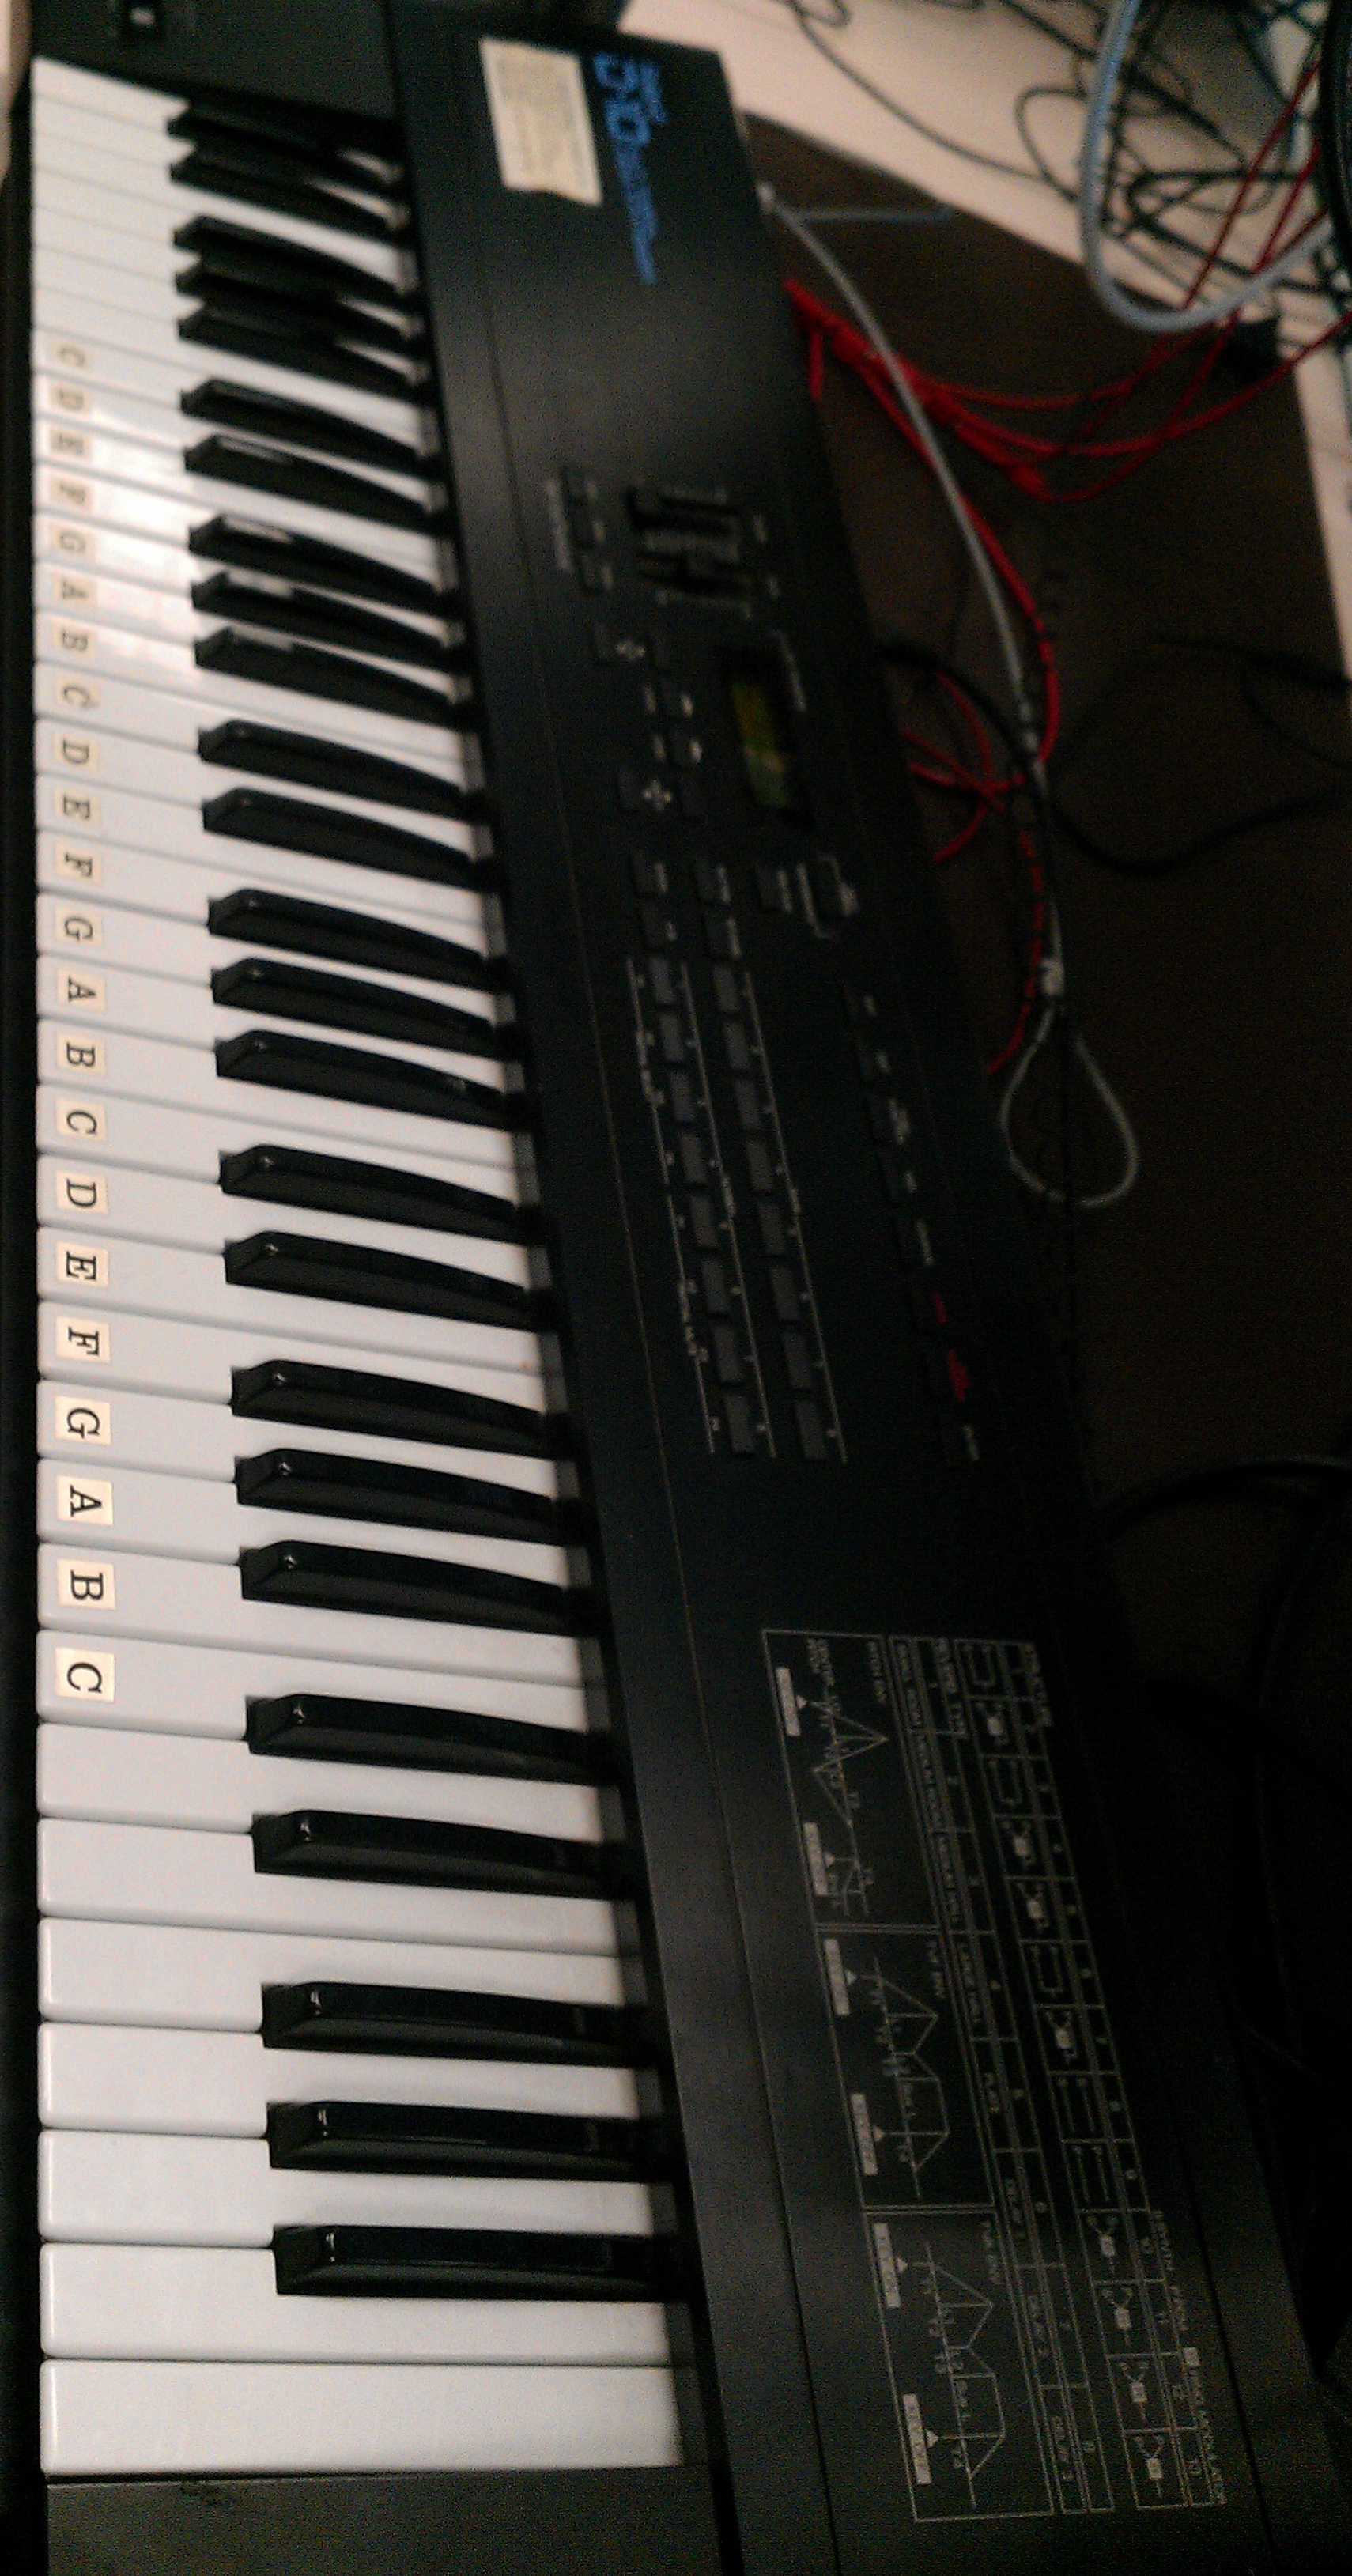
\includegraphics[height=0.47\textheight]{keyboard}\\
    \end{minipage}
    \begin{minipage}[b]{0.6\linewidth}
      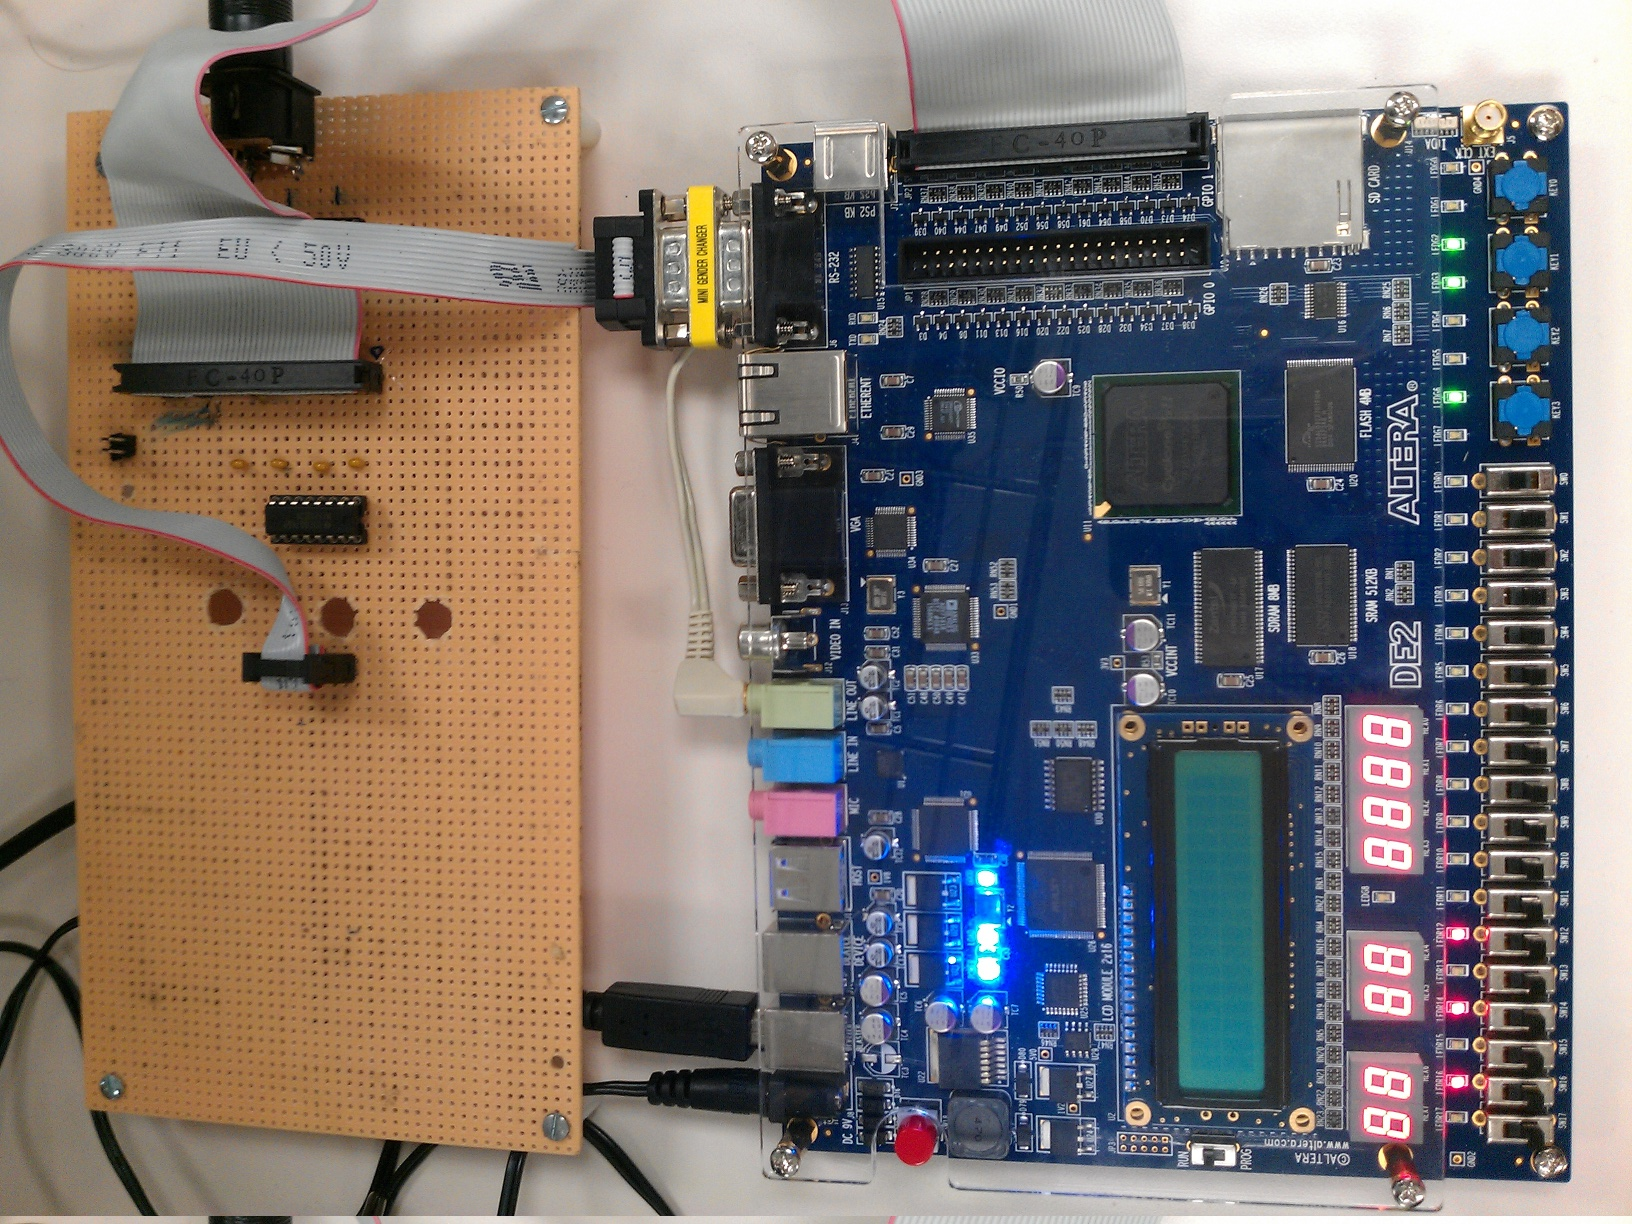
\includegraphics[height=0.47\textheight]{hardware}\\
    \end{minipage}
  }
  \headerbox{\color{white} Digital Synthesis}{name=topright, column=3, row=0, span=1}{\color{dark}
    \medium
    Sound synthesis in this project is accomplished through Wavetable Lookup Synthesis. This process involves storing a sample waveform in a lookup table, then playing those samples at a varying rate dependant upon what frequency you desire to output.
    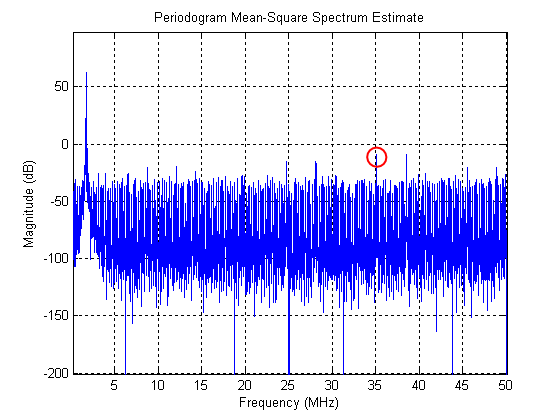
\includegraphics[height=0.25\textheight]{wavetable_freq}\\
  }
  \headerbox{\color{white} Hardware}{name=bottomleft,column=0,above=bottom,span=2}{
    \begin{minipage}[b]{0.55\linewidth}
      \begin{itemize}\color{dark}\medium
        \item MIDI to RS-232 Circuit
        \item Numerically Controller Oscillators
        \item Time-Domain Envelope Generators
        \item Onboard Audio Codec Chip
        \item Onboard Buttons/Switches/LCD
      \end{itemize}
    \end{minipage}
    \begin{minipage}[b]{0.4\linewidth}
      \vspace{0pt}
      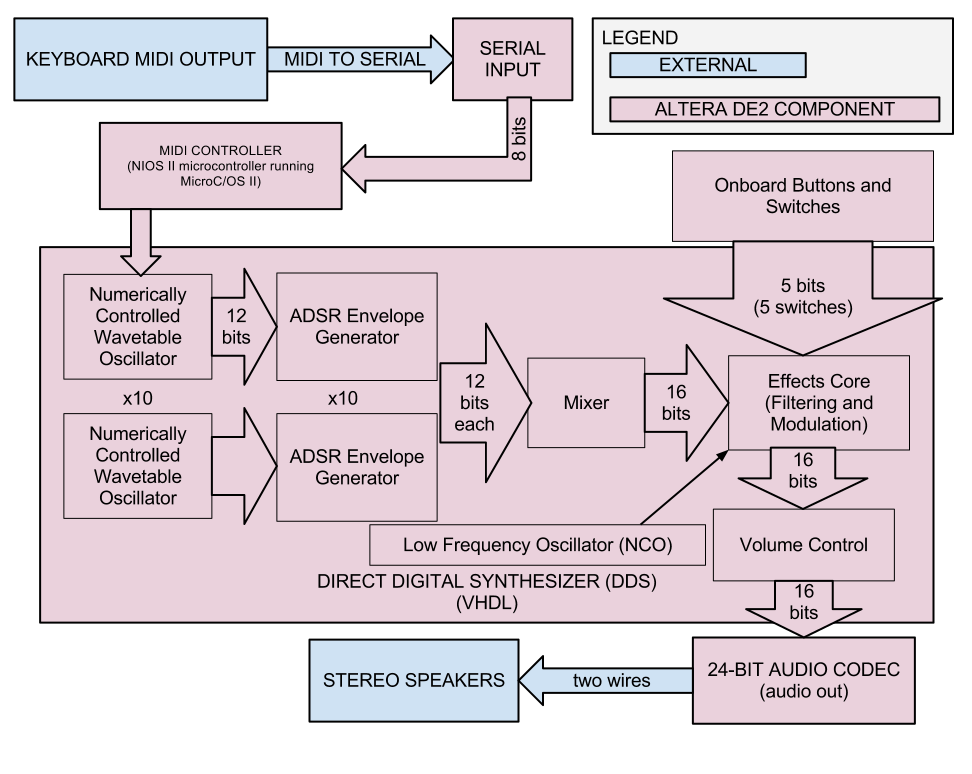
\includegraphics[height=0.23\textheight]{block_diag}
    \end{minipage}
  }
  \headerbox{\color{white} Software}{name=bottomright,column=2,above=bottom,span=2}{\color{dark}\large
    \begin{minipage}[b]{0.43\linewidth}
      \vspace{0pt}
      
\includegraphics[height=0.23\textheight]{software}
    \end{minipage}
    \begin{minipage}[b]{0.52\linewidth}
      \begin{itemize}\color{dark}\medium
        \item uC/OS-II Operating System
        \item Function-Dedicated Tasks
        \item Memory Mapped Interfaces to Hardware
        \item Message Queue Based IPC
      \end{itemize}
    \end{minipage}
  }
\end{poster}%
%
\end{document}
